\documentclass[12pt]{scrartcl}
\usepackage{config}
\usepackage{minted}

%\newcommand\mrh{\color{white}\bfseries}
\newcommand\mrc[1]{\begin{tabular}{@{}l@{}} #1 \end{tabular}}
\setlength\arrayrulewidth{0.8pt}

\usemintedstyle{pastie}

\begin{document}
    \hh{Equipo de investigación de sonrisas}

    
    \vspace{10pt}

    
    \hh{Problema}

        En su odisea para investigar todas las sonrisas del mundo, Rin y Ren han llegado a Ecatepec. Ecatepec puede ser visto como un grafo con $N$ vértices, numerados del $0$ al $N - 1$, conectados por algunas aristas bidireccionales, pero a ser una tierra en gran medida desconocida, el equipo no sabe sobre sus aristas. Si Ecatepec resulta ser no conexo\footnote{Decimos que un grafo es conexo si para todo par de vértices, existe un camino (un camino es una secuencia de vértices, tal que cada par de vértices adyacentes está conectado por una arista) que inicie en uno y termine en otro.}, Rin y Ren no podrán llevar a cabo su misión apropiadamente, por lo que enlistan la ayuda de la gran científica Miku. Miku le da a nuestros aventureros un curioso aparato que responde preguntas de la siguiente forma dado un parámetro $K$ que Miku ha fijado con anterioridad:

        Dados dos vértices distintos de la gráfica de Ecatepec, el aparato responde si están a distancia\footnote{La distancia de dos vértices se define como el camino con menor cantidad de aristas que los conecta, y la expresamos como $dist(a, b)$.} menor a $K$, exactamente $K$ o mayor a $K$.

        Como el dispositivo es todavía un prototipo, Miku le advierte al equipo que podrán realizar a lo más $\frac{2N^2}{K}$ preguntas. Rin y Ren reprobaron matemáticas en la prepa, por lo que enlistan tu ayuda para saber si Ecatepec es conexo.
        

        
    \hh{Detalles de Implementación}

        Debes implementar la función \textit{Equipo\_sonrisas()}. Esta función recibe un entero $N$ el tamaño del grafo y un entero $K$ el parámetro del dispositivo. Esta función debe regresar un par de enteros, si el grafo es conexo debe regresar la pareja $(-1, -1)$. Si el grafo es no conexo, debe regresar una pareja de vértices entre los cuales no exista un camino. 
        
        Durante tu programa, puedes llamar la función \textit{Dispositivo\_Miku()}. Esta función recibe 2 enteros $a, b$ y regresa $-1$ si $dist(a, b) < K$ , $0$ si $dist(a, b) = K$ y $1$ si $dist(a, b) > K$.
        Para poder llamar esta función, debes incluir la librería \textit{``Sonrisas.h"} con el comando \textit{ \#include ``Sonrisas.h" }.
        Un ejemplo de programa se vería así:

\begin{minted}{c++}
#include "Sonrisas.h"
#include <bits/stdc++.h>
using namespace std;

pair<int, int> Equipo_Sonrisas(int N, int K) {
    // Implementa esta función.
}

\end{minted}

    El evaluador llamará esa función \textbf{múltiples} veces por cada caso.
    
    \hh{Ejemplo}

        \begin{itemize}
            \item El evaluador llama la función 
            \begin{center}
                \textit{Equipo\_sonrisas(5, 2)}
            \end{center}
            El grafo escondido es el siguiente:
            \begin{center}
                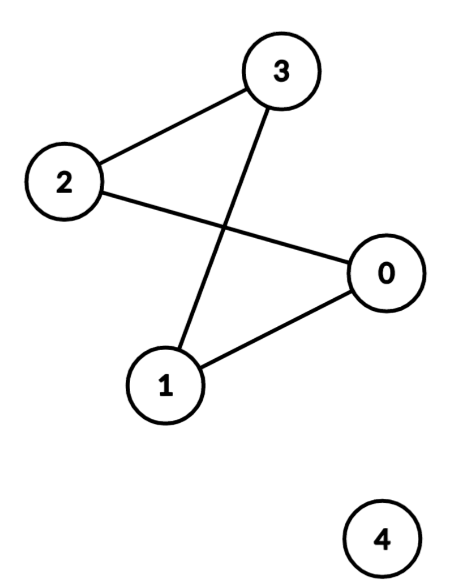
\includegraphics[scale=0.3]{ej1.png}
            \end{center}
            \item La tabla de distancias es la siguiente:
            
            \begin{center}
                \begin{tabular}{|c||c|c|c|c|c|}
                    \hline
                    $dist(a, b)$ & 0 & 1 & 2 & 3 & 4 \\
                    \hline
                    \hline
                     0 & 0 & 1 & 1 & 2 & $\infty$ \\
                     \hline
                     1 & 1 & 0 & 2 & 1 & $\infty$ \\
                     \hline
                     2 & 1 & 2 & 0 & 1 & $\infty$ \\
                     \hline
                     3 & 2 & 1 & 1 & 0 & $\infty$ \\
                     \hline
                     4 & $\infty$ & $\infty$ & $\infty$ & $\infty$ & 0 \\
                     \hline 
                \end{tabular}
            \end{center}
            \item Aquí hay un ejemplo de interacción:
            \begin{center}
                \begin{tabular}{|c|c|}
                    \hline
                     Función llamada & respuesta del evaluador \\
                     \hline 
                     \hline 
                     \textit{Dispositivo\_Miku(0, 1)} & -1 \\
                     \hline 
                     \textit{Dispositivo\_Miku(0, 2)} & -1 \\
                     \hline 
                     \textit{Dispositivo\_Miku(0, 3)} & 0 \\
                     \hline 
                     \textit{Dispositivo\_Miku(0, 4)} & 1 \\
                     \hline 
                     \textit{Dispositivo\_Miku(1, 2)} & 0 \\
                     \hline 
                     \textit{Dispositivo\_Miku(1, 3)} & -1 \\
                     \hline 
                     \textit{Dispositivo\_Miku(1, 4)} & 1 \\
                     \hline 
                     \textit{Dispositivo\_Miku(2, 3)} & -1 \\
                     \hline 
                     \textit{Dispositivo\_Miku(2, 4)} & 1 \\
                     \hline 
                     \textit{Dispositivo\_Miku(3, 4)} & 1 \\
                     \hline 
                \end{tabular}
            \end{center}
            \item La función llamada por el evaluador, en este momento, si responde $(-1, -1)$ obtendría un veredicto de respuesta incorrecta. De lo contrario, si responde, por ejemplo, $(1, 4)$, obtendría un veredicto aceptado.
        \end{itemize}
        
    \hh{Consideraciones}
        \begin{itemize}
            \item $1 \le K < N \le 1000$.
            \item En todos los casos, la cantidad de veces que llamas la función \textit{Dispositivo\_Miku()} debe ser menor a $\frac{2N^2}{K}$. En caso contrario, recibirás un veredicto de respuesta incorrecta.
            \item Si la función regresa $(-1, -1)$ y el grafo es no conexo, o si regresa una pareja de nodos conectados, recibirás un veredicto de respuesta incorrecta.
            \item Sea $S_N$ la suma de los valores de $N$ por cada llamada que haga el evaluador en un caso. Se garantiza que $S_N \le 1000$.
        \end{itemize}
    
    \hh{Subtareas}

    \begin{itemize}
        \item (5 puntos) $K = N - 1$.
        \item (10 puntos) $K \le 4$.
        \item (33 puntos) $K = \frac{N}{2}$.
        \item (22 puntos) El grafo es un bosque (no existe un ciclo, es decir, un camino que no reutilice aristas y comience y termine en el mismo vértice).
        \item (30 puntos) Sin restricciones adicionales.
    \end{itemize}
\end{document}
